\section{Theoretical framework}

\subsection{Graph theory}
This section contains definitions, notation and concepts related to Graph Theory according
to \cite{graph_theory:2010}. \\
Graph theory deals with connection amongst vertices by edges. \\
Graphs are the foundation of many day to day processes and concepts, as they provide a convenient
and intuitive way of representing objects.

\subsubsection{Simple graphs}
A \textbf{simple graph} \textit{G} consists of a non-empty finite set \textit{V(G)} of elements called \textbf{vertices}
(or \textbf{nodes}), and a finite set \textit{E(G)} of distinct unordered pairs of distinct elements of \textit{V(G)}
called \textbf{edges}. We call \textit{V(G)} the \textbf{vertices set} and \textit{E(G)} the \textbf{edge set} of G.
An edge $\{\textit{v}, \textit{w}\}$ is said to \textbf{join} the vertices v and w, and is usually abbreviated to vw. For example, Figure~\ref{fig:simple_graph} represents the simple graph G whose vertex set \textit{V(G)} is $\{\textit{u}, \textit{v}, \textit{w}, \textit{z}\}$, and whose
edge set \textit{E(G)} consists of the edges \textit{uv}, \textit{uw}, \textit{vw} and \textit{wz}. 

\begin{figure}[H]
    \centering
    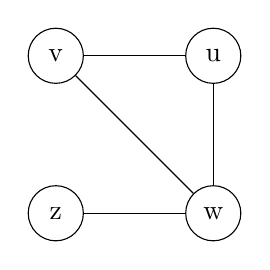
\begin{tikzpicture}
      % Disegno dei nodi
      \node[circle, draw, minimum size=0.7cm] (v) at (0,0) {v};
      \node[circle, draw, minimum size=0.7cm] (u) at (2,0) {u};
      \node[circle, draw, minimum size=0.7cm] (w) at (2,-2) {w};
      \node[circle, draw, minimum size=0.7cm] (z) at (0,-2) {z};
      
      % Disegno degli archi
      \draw (u) -- (v);
      \draw (u) -- (w);
      \draw (v) -- (w);
      \draw (w) -- (z);
    \end{tikzpicture}
    \caption{}
    \label{fig:simple_graph}
\end{figure}

\subsubsection{Adjacency}
We say that two vertices \textit{v} and \textit{w} of a graph \textit{G} are \textbf{adjacent} if there is an edge \textit{vw} joining them, and the vertices \textit{v} and \textit{w} are then \textbf{incident} with such an edge. \\
Similarly, two distinct edges \textit{e} and \textit{f} are \textbf{adjacent} if they have a vertex in common (see Figure \ref{fig:adiacency}).

\begin{figure}[H]
    \centering
    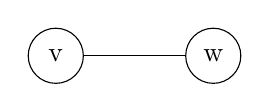
\begin{tikzpicture}
      % Primo grafo
      \node[circle, draw, minimum size=0.7cm] (v) at (0,0) {v};
      \node[circle, draw, minimum size=0.7cm] (w) at (2,0) {w};
      \draw (v) -- (w);
    \end{tikzpicture}
    \quad % Spazio tra i grafi
    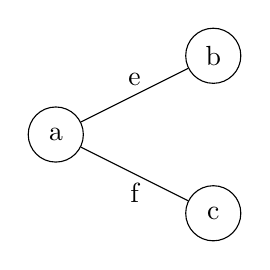
\begin{tikzpicture}
      % Secondo grafo
      \node[circle, draw, minimum size=0.7cm] (a) at (0,0) {a};
      \node[circle, draw, minimum size=0.7cm] (b) at (2,1) {b};
      \node[circle, draw, minimum size=0.7cm] (c) at (2,-1) {c};
      \draw (a) -- node[above] {e} (b);
      \draw (a) -- node[below] {f} (c);
    \end{tikzpicture}
    \caption{Adjacent vertices and adjacent edges}
    \label{fig:adiacency}
\end{figure}

\subsubsection{Matrix representations}
Although it is convenient to represent a graph by a diagram of points joined by lines,
such a representation may be unsuitable if we wish to store a large graph in a computer.
One way of storing a simple graph is involve matrices. \\
Let's consider a graph \textit{G} with \textit{n} vertices and \textit{m} edges. \\
An \textbf{adjacency matrix A} is the $n \times n$ matrix whose \textit{ij}-th entry is the number of edges joining vertex \textit{i} and vertex \textit{j}. \\
If, in addition, the edges are labelled $\{1, 2, \dots, m\}$, its \textbf{incidence matrix M} is the $n \times m$ matrix whose \textit{ij}-th entry is 1 if vertex \textit{i} is incident to edge \textit{j}, and 0 otherwise. \\
An example of this is given in Figure \ref{fig:matrix_representations}.

\begin{figure}[H]
    \centering
    \begin{minipage}{0.5\textwidth}
        \centering
        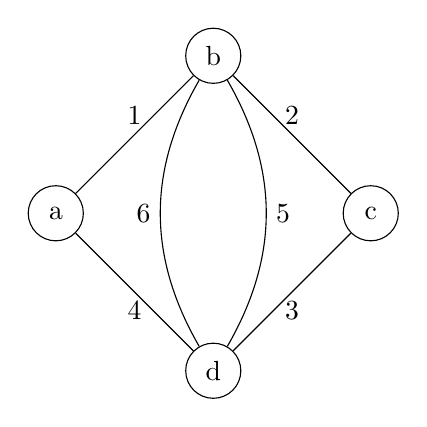
\begin{tikzpicture}
            % Nodi
            \node[circle, draw, minimum size=0.7cm] (a) at (0,0) {a};
            \node[circle, draw, minimum size=0.7cm] (b) at (2,2) {b};
            \node[circle, draw, minimum size=0.7cm] (c) at (4,0) {c};
            \node[circle, draw, minimum size=0.7cm] (d) at (2,-2) {d};
          
            % Archi
            \draw (a) edge node[pos=0.5, below] {4} (d);
            \draw (a) edge node[pos=0.5, above] {1} (b);
            \draw (b) edge[bend left] node[pos=0.5, right] {5} (d);
            \draw (b) edge[bend right] node[pos=0.5, left] {6} (d);
            \draw (b) edge node[pos=0.5, above] {2} (c);
            \draw (c) edge node[pos=0.5, below] {3} (d);
        \end{tikzpicture}
    \end{minipage}%
    \begin{minipage}{0.5\textwidth}
        \[
        A = \begin{bmatrix}
        0 & 1 & 0 & 1 \\
        1 & 0 & 1 & 2 \\
        0 & 1 & 0 & 1 \\
        1 & 2 & 1 & 0
        \end{bmatrix}
        \]
        
        \[
        M = \begin{bmatrix}
        1 & 0 & 0 & 1 & 0 & 0 \\
        1 & 1 & 0 & 0 & 1 & 1 \\
        0 & 1 & 1 & 0 & 0 & 0 \\
        0 & 0 & 1 & 1 & 1 & 1
        \end{bmatrix}
        \]
    \end{minipage}
    \caption{Graph \textit{G} with its adjacency and incidence matrices}
    \label{fig:matrix_representations}
\end{figure}


\subsubsection{Bipartite graphs}
If the vertex set of a graph \textit{G} can be split into two disjoint sets \textit{A} and \textit{B} so that each
edge of \textit{G} joins a vertex of \textit{A} and a vertex of \textit{b}, then \textit{G} is a \textbf{bipartite graph}. \\
Alternatively, a bipartite graph is one whose vertices can be coloured black and white in such a way that each edge joins a black vertex (in \textit{A}) and a white vertex (in \textit{B}). \\
Figure \ref{fig:bipartite} is an example of bipartite graph.

\begin{figure}[H]
    \centering
    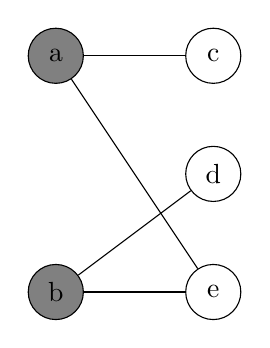
\begin{tikzpicture}[every node/.style={circle, draw, minimum size=0.7cm}]
        % Livello superiore
        \node (A) at (3,0) [fill=black!50] {a};
        \node (B) at (3,-3) [fill=black!50] {b};
        
        % Livello inferiore
        \node (C) at (5,0) [fill=white] {c};
        \node (D) at (5,-1.5) [fill=white] {d};
        \node (E) at (5,-3) [fill=white] {e};
        
        % Collegamenti
        \draw (A) -- (C);
        \draw (A) -- (E);
        \draw (B) -- (D);
        \draw (B) -- (E);
    \end{tikzpicture}
    \caption{}
    \label{fig:bipartite}
\end{figure}



\subsubsection{Bipartite graphs with matching}
A \textbf{bipartite graph with matching} is a bipartite graph in which there is a set of edges selected in such a way that no node is shared among the edges of the matching.
In other words, each node is involved in at most one edge of the matching. \\
This means that if the number of vertices in \textit{A} and \textit{B} is different, at least one vertex will have no connection to another vertex (see Figure \ref{fig:match_1}). \\
If there is the same number of vertices in both \textit{A} and \textit{B}, every vertex is connected to another vertex (see Figure \ref{fig:match_2}). \\
 
\begin{figure}[H]
    \centering
    \begin{minipage}{0.45\textwidth}
        \centering
        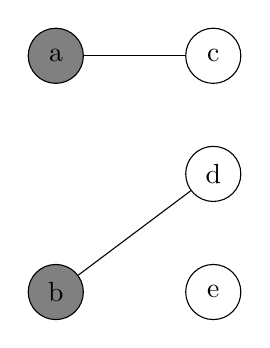
\begin{tikzpicture}[every node/.style={circle, draw, minimum size=0.7cm}]
            % Livello superiore
            \node (A) at (3,0) [fill=black!50] {a};
            \node (B) at (3,-3) [fill=black!50] {b};

            % Livello inferiore
            \node (C) at (5,0) [fill=white] {c};
            \node (D) at (5,-1.5) [fill=white] {d};
            \node (E) at (5,-3) [fill=white] {e};

            % Collegamenti
            \draw (A) -- (C);
            \draw (B) -- (D);
        \end{tikzpicture}
        \caption{}
        \label{fig:match_1}
    \end{minipage}
    \hfill
    \begin{minipage}{0.45\textwidth}
        \centering
        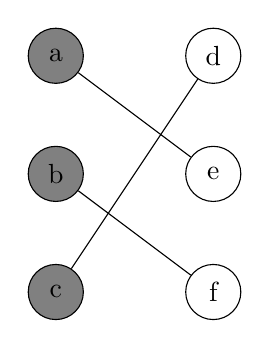
\begin{tikzpicture}[every node/.style={circle, draw, minimum size=0.7cm}]
            % Livello superiore
            \node (A) at (3,0) [fill=black!50] {a};
            \node (B) at (3,-1.5) [fill=black!50] {b};
            \node (C) at (3,-3) [fill=black!50] {c};

            % Livello inferiore
            \node (D) at (5,0) [fill=white] {d};
            \node (E) at (5,-1.5) [fill=white] {e};
            \node (F) at (5,-3) [fill=white] {f};

            % Collegamenti
            \draw (A) -- (E);
            \draw (B) -- (F);
            \draw (C) -- (D);
        \end{tikzpicture}
        \caption{}
        \label{fig:match_2}
    \end{minipage}
\end{figure}

\subsection{Hungarian Algorithm}

The Hungarian matching algorithm, also called the Kuhn-Munkres algorithm, is a \textit{O}($\textit{n}^3$) algorithm that can be used to find maximum-weight matchings in bipartite graphs with \textit{n} vertices for each partition, which is sometimes called the assignment problem.
A bipartite graph can easily be represented by an utility matrix, where the weights of edges are the entries. \\
Come abbiamo già visto nel Brute Force algorithm, i problemi di maximum-weight perfect matching con la matrice di utilità possono essere trasformati in problemi di minimum-weight perfect matching con la matrice di costo.
Spiegheremo l'Hungarian algorithm applicato ai problemi di minimum-weight matching.
\\

\subsubsection{Hungarian Algorithm summarized}

The operation of the Hungarian algorithm for minimum-weigth matching problems can be summerized in these 6 steps:
\begin{enumerate}
    \item {Compute the cost matrix for the considered bipartite graph with \textit{n} vertices in each partition.}
    \item {Subtract the smallest entry in each row from all the other entries in the row. This will make the smallest entry in the row now equal to 0.}
    \item {Subtract the smallest entry in each column from all the other entries in the column. This will make the smallest entry in the column now equal to 0.}
    \item {Draw lines through the row and columns that have the 0 entries such that the fewest lines possible are drawn.}
    \item {If there are n lines drawn, an optimal assignment of zeros is possible and the algorithm is finished. If the number of lines is less than n, then the optimal number of zeroes is not yet reached. Go to the next step.}
    \item {Find the smallest entry not covered by any line. Subtract this entry from each row that isn’t crossed out, and then add it to each column that is crossed out. Then, go back to Step 3.}
\end{enumerate}

\subsubsection{Hungarian Algorithm application}

Let's take for example the same cost matrix of the Brute Force example and try to apply the Hungarian algorithm for minimum-weigth matching problems:

\begin{table}[H]
\centering
\begin{tabular}{|>{\centering\arraybackslash}m{0.6cm}|>{\centering\arraybackslash}m{0.6cm}|>{\centering\arraybackslash}m{0.6cm}|}
  \hline
  108 & 125 & 150 \\
  \hline
  150 & 135 & 175 \\
  \hline
  122 & 148 & 250 \\
  \hline
\end{tabular}
\end{table}

Subtract the smallest value in each row from the other values in the row:

\begin{table}[H]
\centering
\begin{tabular}{|>{\centering\arraybackslash}m{0.6cm}|>{\centering\arraybackslash}m{0.6cm}|>{\centering\arraybackslash}m{0.6cm}|}
  \hline
  0 & 17 & 42 \\
  \hline
  15 & 0 & 40 \\
  \hline
  0 & 26 & 128 \\
  \hline
\end{tabular}
\end{table}

Now, subtract the smallest value in each column from all other values in the column:

\begin{table}[H]
\centering
\begin{tabular}{|>{\centering\arraybackslash}m{0.6cm}|>{\centering\arraybackslash}m{0.6cm}|>{\centering\arraybackslash}m{0.6cm}|}
  \hline
  0 & 17 & 2 \\
  \hline
  15 & 0 & 0 \\
  \hline
  0 & 26 & 88 \\
  \hline
\end{tabular}
\end{table}

There are 2 lines drawn, and 2 is less than 3, so there is not yet the optimal number of zeroes.

\begin{table}[H]
\centering
\begin{tabular}{|>{\centering\arraybackslash}m{0.6cm}|>{\centering\arraybackslash}m{0.6cm}|>{\centering\arraybackslash}m{0.6cm}|}
  \hline
  \cellcolor{gray!25} 0 & 17 & 2 \\
  \hline
  \cellcolor{gray!25} 15 & \cellcolor{gray!25} 0 & \cellcolor{gray!25} 0 \\
  \hline
  \cellcolor{gray!25} 0 & 26 & 88 \\
  \hline
\end{tabular}
\end{table}

Find the smallest entry not covered by any line. Subtract this entry from each row that isn’t crossed out, and then add it to each column that is crossed out. Then, go back to Step 3.
2 is the smallest entry.
First, subtract from the uncovered rows:

\begin{table}[H]
\centering
\begin{tabular}{|>{\centering\arraybackslash}m{0.6cm}|>{\centering\arraybackslash}m{0.6cm}|>{\centering\arraybackslash}m{0.6cm}|}
  \hline
  \cellcolor{gray!25} -2 & 15 & 0 \\
  \hline
  \cellcolor{gray!25} 15 & \cellcolor{gray!25} 0 & \cellcolor{gray!25} 0 \\
  \hline
  \cellcolor{gray!25} -2 & 24 & 86 \\
  \hline
\end{tabular}
\end{table}

Now add to the covered columns:

\begin{table}[H]
\centering
\begin{tabular}{|>{\centering\arraybackslash}m{0.6cm}|>{\centering\arraybackslash}m{0.6cm}|>{\centering\arraybackslash}m{0.6cm}|}
  \hline
  \cellcolor{gray!25} 0 & 15 & 0 \\
  \hline
  \cellcolor{gray!25} 17 & \cellcolor{gray!25} 0 & \cellcolor{gray!25} 0 \\
  \hline
  \cellcolor{gray!25} 0 & 24 & 86 \\
  \hline
\end{tabular}
\end{table}

Now go back to step 3, drawing lines through the rows and columns that have 0 entries:

\begin{table}[H]
\centering
\begin{tabular}{|>{\centering\arraybackslash}m{0.6cm}|>{\centering\arraybackslash}m{0.6cm}|>{\centering\arraybackslash}m{0.6cm}|}
  \hline
  \cellcolor{gray!25} 0 & \cellcolor{gray!25} 15 & \cellcolor{gray!25} 0 \\
  \hline
  \cellcolor{gray!25} 17 & \cellcolor{gray!25} 0 & \cellcolor{gray!25} 0 \\
  \hline
  \cellcolor{gray!25} 0 & 24 & 86 \\
  \hline
\end{tabular}
\end{table}

There are 3 lines (which is nn), so we are done. The assignment will be where the 0's are in the matrix such that only one 0 per row and column is part of the assignment.

\begin{table}[H]
  \centering
  \begin{tabular}{|>{\centering\arraybackslash}m{0.6cm}|>{\centering\arraybackslash}m{0.6cm}|>{\centering\arraybackslash}m{0.6cm}|}
    \hline
    0 & 15 & \cellcolor{yellow!25} 0 \\
    \hline
    17 & \cellcolor{yellow!25} 0 & 0 \\
    \hline
    \cellcolor{yellow!25} 0 & 24 & 86 \\
    \hline
  \end{tabular}
  \end{table}

Replace the original values:

\begin{table}[H]
\centering
\begin{tabular}{|>{\centering\arraybackslash}m{0.6cm}|>{\centering\arraybackslash}m{0.6cm}|>{\centering\arraybackslash}m{0.6cm}|}
  \hline
  108 & 125 & \cellcolor{yellow!25} 150 \\
  \hline
  150 & \cellcolor{yellow!25} 135 & 175 \\
  \hline
  \cellcolor{yellow!25} 122 & 148 & 250 \\
  \hline
\end{tabular}
\end{table}

We find that the minimum total cost is given by this assignment.

\subsection{Game theory}
Game theory is a type of decision theory in which one’s choice of action is determined after taking
into account all possible alternatives available to an opponent playing the same game, rather than just
by the possibilities of several outcome results. \\
Game theory does not insist on how a game should be played but tells the procedure and principles by which action should be selected.
Thus it is a decision theory useful in competitive situations. \\
Game is defined as an activity between two or more persons according to a set of rules at the end of
which each person receives some benefit or suffers loss. The set of rules defines the game.
Going through the set of rules once by the participants defines a play.
\\

The following sections contains notations and properties accordind to \cite{game_theory:2020}.

\subsubsection{Properties of a Game}
\begin{enumerate}
    \item {There are finite numbers of competitors called \textit{players}.}
    \item {Each player has a finite number of possible courses of action called \textit{strategies}.}
    \item {All the strategies and their effects are known to the players but player does not know which
    strategy is to be chosen.}
    \item {A game is played when each player chooses one of his strategies. The strategies are assumed
    to be made simultaneously with an outcome such that no player knows his opponents strategy
    until he decides his own strategy.}
    \item {The game is a combination of the strategies and in certain units which determines the gain or
    loss.}
    \item {The figures shown as the outcomes of strategies in a matrix form are called \textit{pay-off matrix}.}
    \item {The player playing the game always tries to choose the best course of action which results in
    optimal pay off called \textit{optimal strategy}.}
    \item {The expected pay off when all the players of the game follow their optimal strategies is
    known as \textit{value of the game}. The main objective of a problem of a game is to find the value
    of the game.}
    \item {The game is said to be \textit{fair} game if the value of the game is zero otherwise it's known as \textit{unfair}.}
    \item {A \textit{coalition} is a subset of the players \textit{n}, whereas a \textit{grand coalition} is the
        set \textit{n} of all players. The purpose of a coalition is to coordinate strategies and divide the
        total payoff among all the players.}
\end{enumerate}


\subsubsection{Cooperative Games}
A cooperative game is a situation in which players interact together to achieve a common goal.
In the context of a cooperative game, players aim to maximize the overall outcome by collaborating, communicating, and coordinating their actions.
The primary objective is to achieve a result in which all players benefit, working together to overcome challenges or issues.


\subsubsection{Non-cooperative Games}
A non-cooperative game is a situation in which players act independently and without direct communication or coordination with other players.
In a non-cooperative game, each player seeks to maximize their individual gain without necessarily considering the effect of their actions on other players.
The main goal is to achieve the best personal outcome, even at the expense of other participants, without considering direct collaboration.


\subsubsection{The Prisoner's Dilemma}
The Prisoner's Dilemma is a fundamental concept in game theory that illustrates the challenges of \textit{cooperation} and \textit{non-cooperation} between individuals. \\
It's a model that exemplifies situations where two individuals could benefit from collaboration, but are tempted to act selfishly to maximize their personal gains. \\
Here's how it works:
\\

\textbf{Scenario:}
Imagine two criminals (\textit{A} and \textit{B}) who have been arrested and are held in separate cells. \\
There is not enough evidence to convict them for the most serious crime, but there is enough evidence to convict them for a lesser crime.
Both of them are offered the opportunity to \textit{confess} (\textit{betray}) or \textit{remain silent} (\textit{cooperate}).
\\

\textbf{Options:}
\begin{enumerate}
    \item {If \textit{both remain silent}, they each receive a short sentence of 1 year for the lesser crime.}
    \item {If \textit{one of them betrays} and \textit{the other cooperates}, the betrayer will be released without any sentence, and the other will receive a long sentence of 3 years.}
    \item {If \textit{both betray}, they both receive a moderate sentence of 2 years for the lesser crime, which is longer than if they both cooperate.}
\end{enumerate}

\begin{figure}[H]
    \centering
    \begin{minipage}{0.5\textwidth}
        \centering
        \begin{tabular}{|c|c|c|}
        \hline
        \backslashbox{A}{B} & Silence & Betray \\
        \hline
        Silence & \backslashbox{1}{1} & \backslashbox{3}{0} \\
        \hline
        Betray & \backslashbox{0}{3} & \backslashbox{2}{2} \\
        \hline
        \end{tabular}
        \caption{Years for crimanal \textit{A} and \textit{B}}
        \label{tab:contingency_table_1}
    \end{minipage}%
    \begin{minipage}{0.5\textwidth}
        \centering
        \begin{tabular}{|c|c|c|}
        \hline
        \backslashbox{A}{B} & Silence & Betray \\
        \hline
        Silence & 2 & 3 \\
        \hline
        Betray & 3 & 4 \\
        \hline
        \end{tabular}
        \caption{Total years for the group of criminals}
        \label{tab:contingency_table_2}
    \end{minipage}
    \end{figure}
    

\textbf{Outcomes:}
\begin{itemize}[label=\textbullet]
    \item If both act rationally to maximize their own gain, the most likely outcome is that both will betray, leading to a moderate sentence for both. This is the non-cooperative result.
    \item However, if both trust each other and cooperate, they would achieve the best possible outcome for both: the shortest sentence.
\end{itemize}


\textbf{Implications:} The Prisoner's Dilemma demonstrates how even though cooperating would be in their collective interest, the two prisoners might be tempted to betray each other to avoid a longer sentence. \\
This conflict between personal benefit and the common good often leads to suboptimal outcomes. \\
The Prisoner's Dilemma has been extensively studied in psychology, economics, and social sciences and is a crucial example of the challenges of cooperation in human interactions. \\


\subsection{Machine Learning Theory}
Machine Learning deals with the ability of a system to improve its performance through experience, without being explicitly programmed.
It also serves as the foundation for numerous everyday applications and concepts, 
as it provides a powerful and efficient way to address complex challenges, make data-driven decisions, 
and develop intelligent systems that can learn and adapt autonomously.\\

Diving deeper into this concept, one critical aspect is the role of hyperparameters. 
Hyperparameters are settings or configurations that guide the learning process of machine learning algorithms. 
They act as the levers that fine-tune the behavior of these algorithms, influencing their performance, accuracy, and generalization capabilities.\\
Hyperparameters encompass a wide range of choices, such as the learning rate in gradient descent, the depth of a decision tree, the number of hidden layers in a neural network, or the number of clusters in a k-means clustering algorithm. 
Selecting the right hyperparameters can be a challenging and often iterative task, as they significantly impact the model's ability to capture underlying patterns in data.\\
The process of hyperparameter tuning involves experimenting with different combinations of values, assessing the model's performance using techniques like cross-validation, and iteratively adjusting the hyperparameters to optimize the model's accuracy and generalization. 
This fine-tuning is crucial to ensure that the machine learning model not only fits the training data well but also performs effectively on unseen data.
Moreover, the choice of hyperparameters is problem-dependent, and there's no one-size-fits-all solution. 
It requires a deep understanding of the algorithm, the dataset, and the specific problem at hand.

\subsubsection{Classifier}
A mathematical \textbf{Classifier} is a model that takes an input dataset and assigns each data point to a class or category. 
The mathematical formulation of a classifier can vary depending on the algorithm used. 
Suppose we have a training dataset represented as pairs (\textit{$\overline{x}$}, \textit{y}), where \textit{$\overline{x}$} is a vector of data features, and \textit{y} is the associated class label.
The \textit{y} is a categorical (can take a fixed, number of possible values) variable that categorizes between two or more classes ('dog', 'cat', 'bird'), while in a regression problem it is a continuous variable.
Our goal is to find a function \textit{f}(\textit{$\overline{x}$}) that maps the feature vectors \textit{$\overline{x}$} to class labels \textit{y}. 


\subsubsection{K-Nearest Neighbors}
The \textbf{KNN} algorithm is a supervised machine learning algorithm used for classification and regression tasks.
It is a simple and intuitive algorithm that makes predictions based on the similarity between a data point and its k-nearest neighbors in a training dataset.
The \textit{k} in \textit{k}-nearest neighbors refers to the number of items that the algorithm uses to make its prediction whether its a classification problem or a regression problem.
In Figure \ref{fig:knn} we can see a test sample represented by a green dot and we want to classify 
it either as a blue square or a red triangle based on a KNN algorithm, the decision depends on the value of \textit{k}, which determines how many nearest neighbors we consider.\\
When \textit{k} = 3 (solid line circle), the green dot is assigned to the category that has the majority among its three nearest neighbors. 
In this case, if there are 2 red triangles and only 1 blue square inside the inner circle, the green dot is classified as a red triangle. \\
When \textit{k} = 5 (dashed line circle), the green dot is assigned to the category with the majority among its five nearest neighbors. 
If there are 3 blue squares and 2 red triangles inside the outer circle, the green dot is classified as a blue square.
\begin{figure}[H]
    \centering
    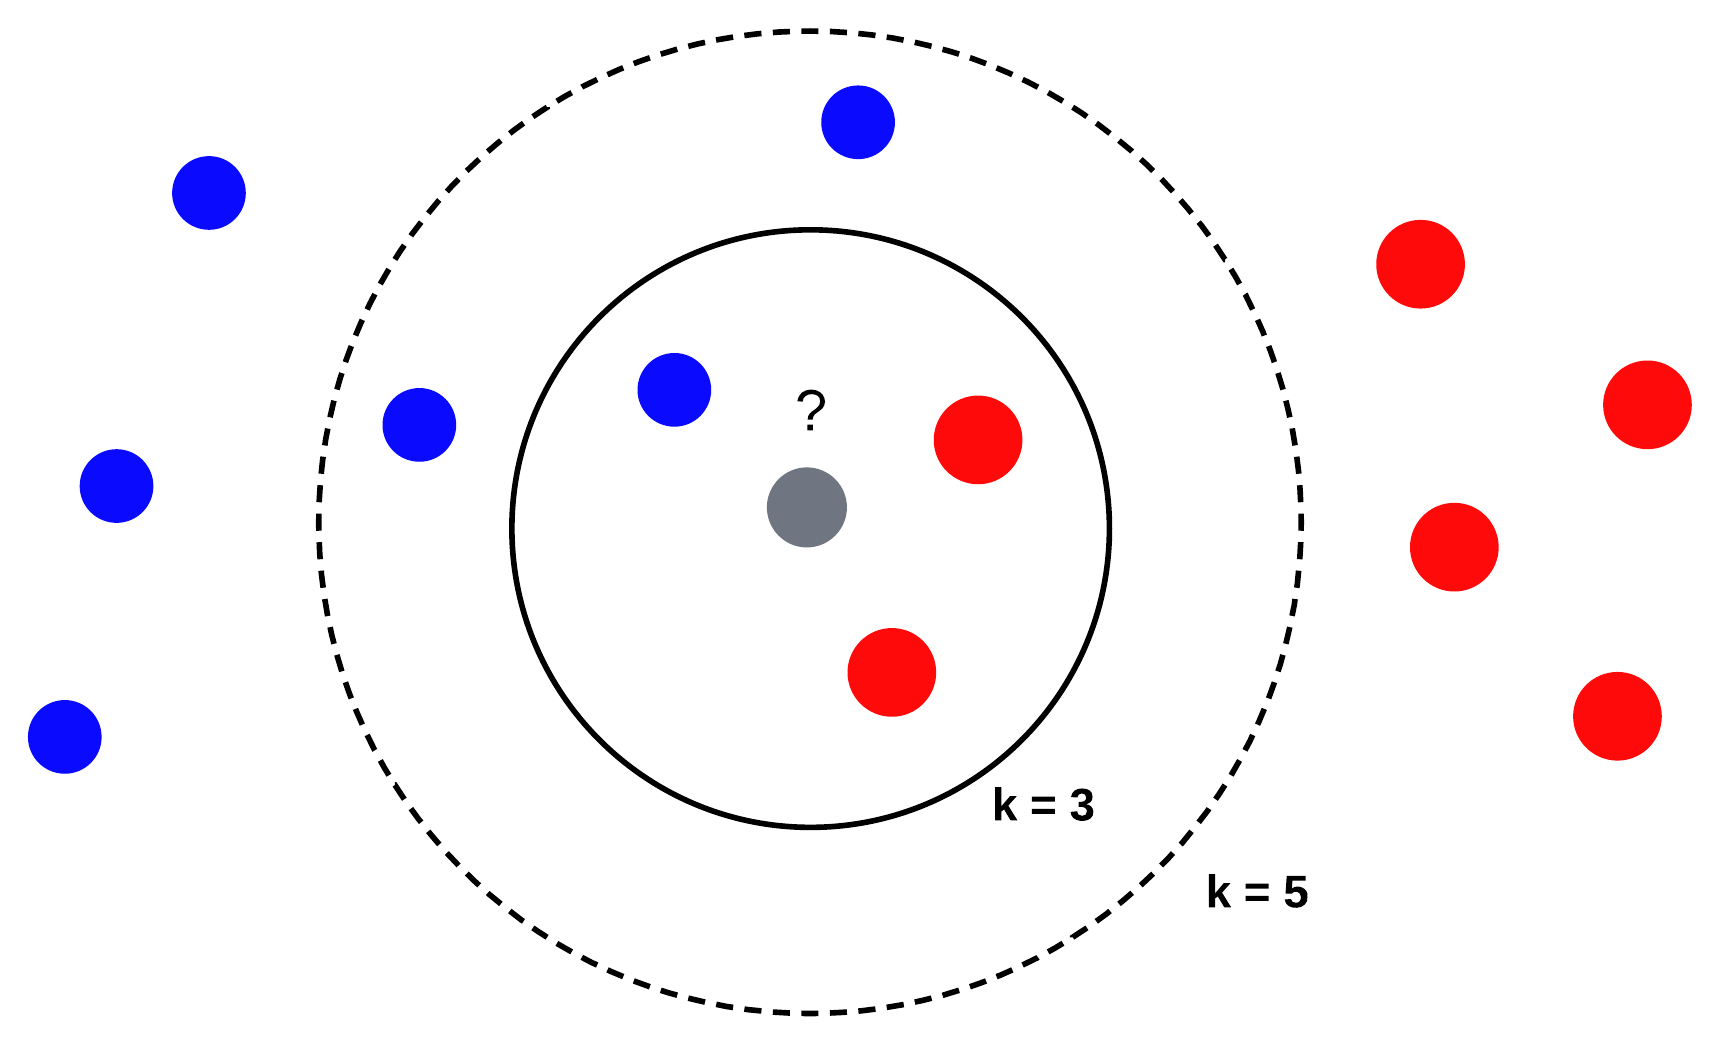
\includegraphics[width=0.6\linewidth]{graphics/KNeighbours.png}
    \caption{KNN algorithm with \textit{k} = 3 and \textit{k} = 5}
    \label{fig:knn}
\end{figure}

The choice of distance metric is a critical aspect of the KNN algorithm, and while it's not typically considered a hyperparameter, it significantly influences the model's performance and outcomes. 
The selection of a specific distance metric can have a substantial impact, especially when dealing with datasets of varying sizes and dimensions. \\
If we consider for example two data points \textit{p}, \textit{q} in \textit{n}-dimensional space, there are various distance metrics that can be used to find the neighbors.\\
Among the different  most common is the Euclidean distance: 
\begin{center}
    \begin{equation}
        Euclidean(p,q) = \sqrt{\sum_{i=1}^{n} (p_i - q_i)^2}
        \end{equation}
\end{center}

\subsubsection{Borderline Synthetic Minority Over-sampling Technique}
\textbf{Oversampling} is a technique used in the field of imbalanced machine learning to address the problem of class imbalance. 
Class imbalance occurs when one class in a classification problem has significantly fewer instances than another class. 
This imbalance can lead to biased models that perform poorly on the minority class (the class with fewer instances) because the model tends to be biased towards the majority class.\\
The concept of oversampling involves increasing the number of instances in the minority class by generating synthetic or duplicate samples. 
The goal is to balance the class distribution, making the minority class more comparable in size to the majority class. 
A synthetic sample can be generated duplicating randomly another sample of the minority class or considering its underlying data distribution (ADASYN \cite{adasyn:2008}).
This could result in a performance improvement of machine learning models by providing them with more information about the minority class.\\
The SMOTE generates synthetic samples by interpolating between neighboring minority class instances using an underlying KNN model.\\

The \textbf{B-SMOTE} \cite{Han2005BorderlineSMOTEAN:2005}, is a vairant of the SMOTE that focuses on generating synthetic samples only for the boundary instances, which are the minority class instances close to the majority class. 
This approach aims to concentrate on the regions of the dataset that are near the decision boundary between classes. \\
The model internally fits two instances of KNN with different \textit{k} parameters: one instance to defines the neighborhood of samples to generate the synthetic samples.
The other instead is used to determine if a minority sample is in “danger”. A "sample in danger" is one near to the boundary between two or more classes.

In the illustrated scenario depicted in Figure \ref{fig:bordSMOTEnotApplied}, the task involves categorizing two distinct categories of network traffic: 
one being malicious (depicted in red), the other representing legitimate traffic (shown in blue), and the decision boundaries are the same color meshes.
The distribution of malicious traffic is more sparse and rare compared to legitimate traffic, this means that the classifier has been trained on an imbalanced dataset. 
The primary objective of the classification is to maximize the detection of malicious traffic, even if it entails misclassifying some instances of legitimate traffic. 
BSMOTE is a possible solution for this scenario, where the two classes are significantly imbalanced, and the weight of legitimate traffic in the classification process could be overwhelming.

The application of the BSMOTE algorithm facilitates class rebalancing by generating synthetic data points in the boundary regions between the classes concentrated in proximity of the decision boundary.
In Figure \ref{fig:bordSMOTEApplied}, the depicted image showcases the ultimate outcome achieved following the retraining of the classifier. 
The retraining process maintained the same parameters but employed a dataset that has been more uniformly balanced.
The synthetic samples generated by BSMOTE are represented as light-red dots.
\begin{figure}[H]
  \centering
  \begin{subfigure}{0.48\linewidth}
    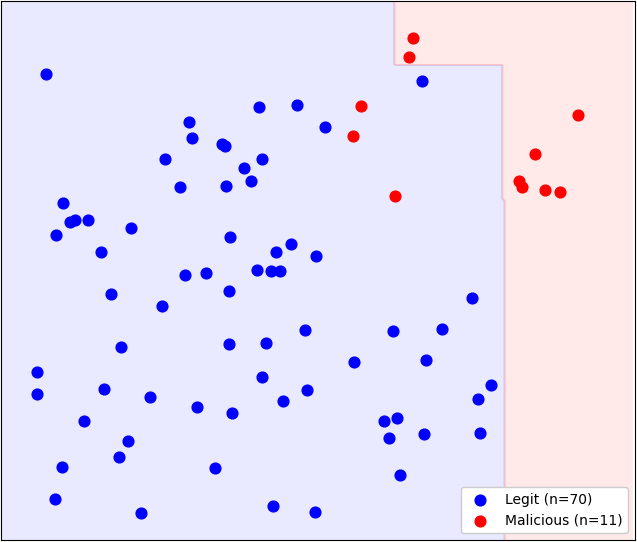
\includegraphics[width=\linewidth]{graphics/BordSMOTE_no.png}
    \caption{}
    \label{fig:bordSMOTEnotApplied}
  \end{subfigure}
  \hspace{0.02\linewidth}
  \begin{subfigure}{0.48\linewidth}
    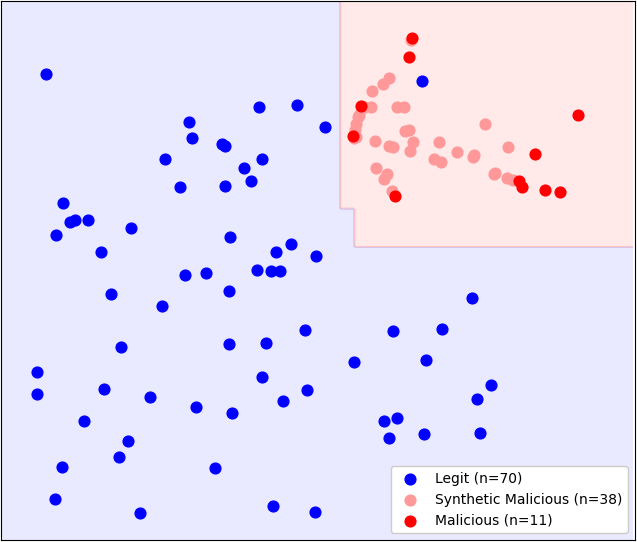
\includegraphics[width=\linewidth]{graphics/BordSMOTE_yes.png}
    \caption{}
    \label{fig:bordSMOTEApplied}
  \end{subfigure}
  \caption{Visual representation of BSMOTE algorithm applied on a dataset}
\end{figure}

However The BSMOTE algorithm, like any other method, has its limitations and drawbacks:
\begin{itemize}
  \item \textbf{Risk of Overfitting:} In the provided example, the malicious data was generated using a normal distribution, while the legitimate data was generated using a uniform distribution.
  This means that the second classification fits better the underlying distribution without any a-priori assumption.
  But in some cases depending on the choice of borderline examples, 
  BSMOTE may introduce a bias towards certain patterns or classes in the synthetic samples, which can affect the model's generalization.
  It can potentially lead to overfitting, especially when it generates a large number of synthetic samples in the borderline region. 
  This may cause the model to perform exceptionally well on the training data but poorly on unseen data.
  \item \textbf{Computationally intensive:} It can require high hardware resources, especially in high-dimensional spaces, as it involves calculating distances between data points. 
  This can lead to longer training times, making it less suitable for large datasets.
  \item \textbf{Designed for Clearly Separable Datasets:} It is designed for datasets with clear class boundaries and is most effective when the borderline instances are well-defined. 
  In cases where class separation is not distinct, it may not provide substantial benefits.
\end{itemize}
So in general, even if it aims to improve the classification of the minority class, there is no guarantee that it will always lead to better results.

\subsubsection{Random Forest Classifier}
A \textbf{Decision Tree} (DT) is a non-parametric supervised learning algorithm, which is utilized for both classification and regression tasks. 
It has a hierarchical, tree structure, which consists of a internal nodes, leaf nodes and branches.
From the root node, splitting criterias are applied on the samples creating branches and child nodes that lead to leaf nodes which represent the final classification of the tree.
The most common impurity measure used to quantify the impurity of a dataset is the Gini criterion:
For a set of items with \textit{J} classes and relative frequencies $p_{i}$, $i \in {1,2,...,J}$ 
the probability of choosing an item with label $i$ is $p_{i}$, and the probability of miscategorizing that item is:
\begin{equation} 
  \sum_{k \ne i} p_{k} = 1 - p_{i} 
\end{equation}
The Gini impurity is computed by summing pairwise products of these probabilities for each class label:
\begin{center}
  \begin{equation}
    Gini(p) = 1 - \sum_{i=1}^{J} (p_i^2)
  \end{equation}
\end{center}

In the example shown in Table \ref{tab:tableDecisionTreeDataset}, the objective is to determine whether to grant a loan based on two pieces of information: 
the applicant's monthly income and the requested loan amount. The second figure illustrates the DT that has been trained on this dataset.
The underlying principle of the DT is that at every non-terminal node, if there exist samples that need further separation, the following algorithm is applied: 
\begin{enumerate}
  \item It starts by calculating the impurity of the current node before making any splits. This initial impurity serves as a baseline for evaluating feature splits.
  \item For each feature in the dataset, calculate a measure of impurity or information gain for potential splits. This typically involves examining the feature values and considering different threshold values.
  \item Calculates the reduction in impurity (or information gain) achieved by the potential split. This is done by comparing the impurity of the current node with the impurity of the child nodes created by the split.
  \item Choose the feature that results in the highest information gain. This feature becomes the one on which to apply the threshold for the split.
  \item It applies the threshold that separates the data into two or more subsets.
  \item Continue the process recursively for each child node created by the split. This means repeating steps 1 to 5 for each child node until a stopping criterion is met (e.g., a maximum tree depth is reached).
\end{enumerate}
The goal is to create child nodes that are as homogeneous as possible with respect to the target variable, thereby improving the predictive accuracy of the tree.
\begin{table}[H]
  \centering
  \begin{tabular}{|>{\centering\arraybackslash}p{3.2cm}|>{\centering\arraybackslash}p{3.2cm}|>{\centering\arraybackslash}p{3.2cm}|}
  \hline
  \textbf{Income} & \textbf{Loan\_Amount} & \textbf{Loan\_Approved} \\
  \hline
  2000 & 300000 & Not Approved \\
  3000 & 300000 & Approved \\
  4000 & 400000 & Not Approved \\
  5000 & 400000 & Not Approved \\
  10000 & 400000 & Approved \\
  15000 & 400000 & Approved \\
  \hline
  \end{tabular}
  \caption{Dataset of the DT}
  \label{tab:tableDecisionTreeDataset}
\end{table}
\begin{figure}[H]
  \centering
  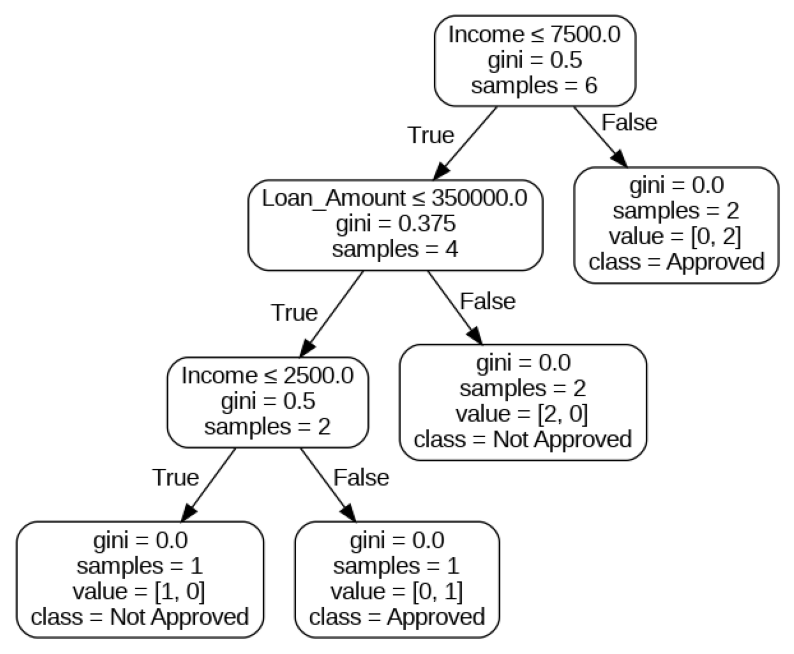
\includegraphics[width=0.7\linewidth]{graphics/DecTree.png}
  \label{fig:knn5}
  \caption{DT applied on the dataset of Table \ref{tab:tableDecisionTreeDataset}}
\end{figure}
Note that due to the absence of constraints on hyperparameters like tree depth or the minimum number of features required to split nodes, 
it becomes evident that each sample in the dataset follows a distinct path within this tree. 
This situation results in a phenomenon known as overfitting, where the model essentially molds itself too closely to the training data.\\

\textbf{Random Forest} (RF) is an ensemble learning method that builds multiple DTs during training and combines their predictions to make more accurate and robust classifications or regressions.
A RF is typically constructed in this way:
\begin{enumerate}
  \item \textbf{Bootstrapped Data:} A random subset of the training data (with replacement) is used to train each DT. This results in each tree being trained on a slightly different dataset.
  \item \textbf{Random Feature Selection:} At each node of each DT, only a random subset of the available features is considered for splitting. This helps introduce diversity among the trees and reduces the risk of overfitting.
  \item \textbf{Independent Training:} Each DT is trained independently. There is no communication or shared information between the trees during training.
  \item \textbf{Voting or Averaging:} For classification tasks, the RF combines the individual tree predictions by applying a Majority Voting (each tree "votes" for a class and the final prediction reflects the class that receives the most votes overall)
\end{enumerate}
The key idea behind the RF method is that by aggregating the predictions of multiple DTs, the ensemble can reduce overfitting, improve generalization, and provide more robust and accurate results.
For example the Figure \ref{fig:rf} is shown a RF classifier made of 3 DTs has been created applying the bootstrap method on the dataset and correctly classifies the first sample of the dataset in Table \ref{tab:tableDecisionTreeDataset}.

\begin{figure}[H]
  \centering
  \begin{subfigure}{0.45\linewidth}
    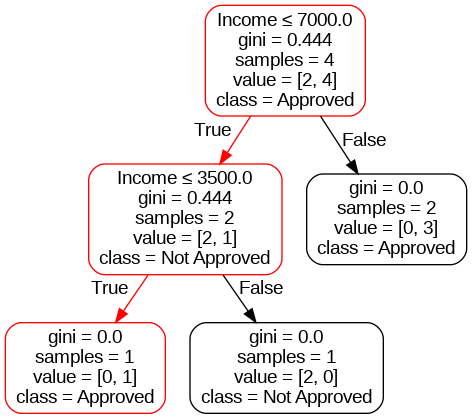
\includegraphics[width=\linewidth]{graphics/loan_RF_1.png}
    \caption{}
    \label{fig:rfTree0}
  \end{subfigure}
  \hspace{0.06\linewidth}
  \begin{subfigure}{0.45\linewidth}
    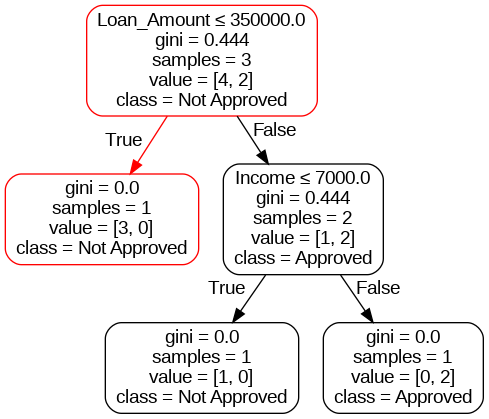
\includegraphics[width=\linewidth]{graphics/loan_RF_2.png}
    \caption{}
    \label{fig:rfTree1}
  \end{subfigure}
  \begin{subfigure}{0.39\linewidth}
    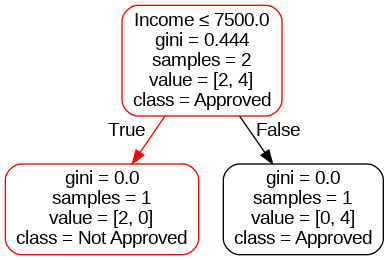
\includegraphics[width=\linewidth]{graphics/loan_RF_0.png}
    \caption{}
    \label{fig:rfTree2}
  \end{subfigure}
  \caption{Path taken by the first sample through the three DTs of a RF classifier}
  \label{fig:rf}
\end{figure}


\subsubsection{Cross Validation}
\textbf{Cross Validation} is a technique used to estimate the effectiveness of a machine learning model based on a data sample.
It involves dividing the dataset into multiple training and testing subsets called \textit{folds} and then training and evaluating the model on each fold.
The process of training and testing is typically repeated multiple times and the results from each iteration are often averaged to provide an overall estimate of the model's performance.
The most common approach in basic cross-validation is to use a 80-20 or 70-30 split between the training and test sets.
This helps ensure that the model is not only learning from the data but also being tested on data it has not seen during training.
\\

\textbf{Leave-One-Out Cross-Validation} (LOOCV) is a specific type of cross validation where the number of folds \textit{k} equals the number of samples in the dataset.\\
The model is trained \textit{k} times, with \textit{k} equal to the total number of samples. \\
At each \textit{k}-iteration, a different sample is selected as the test set, while all the other samples are used for training. \\
LOOCV provides a very accurate estimate of the model's performance because it uses all available data for training and validation.
However, it can be computationally expensive, especially on large datasets, as it requires a significant number of separate model trainings. \\
In Figure \ref{fig:LOOCV} we can see how it works.

\begin{figure}[H]
  \centering  
    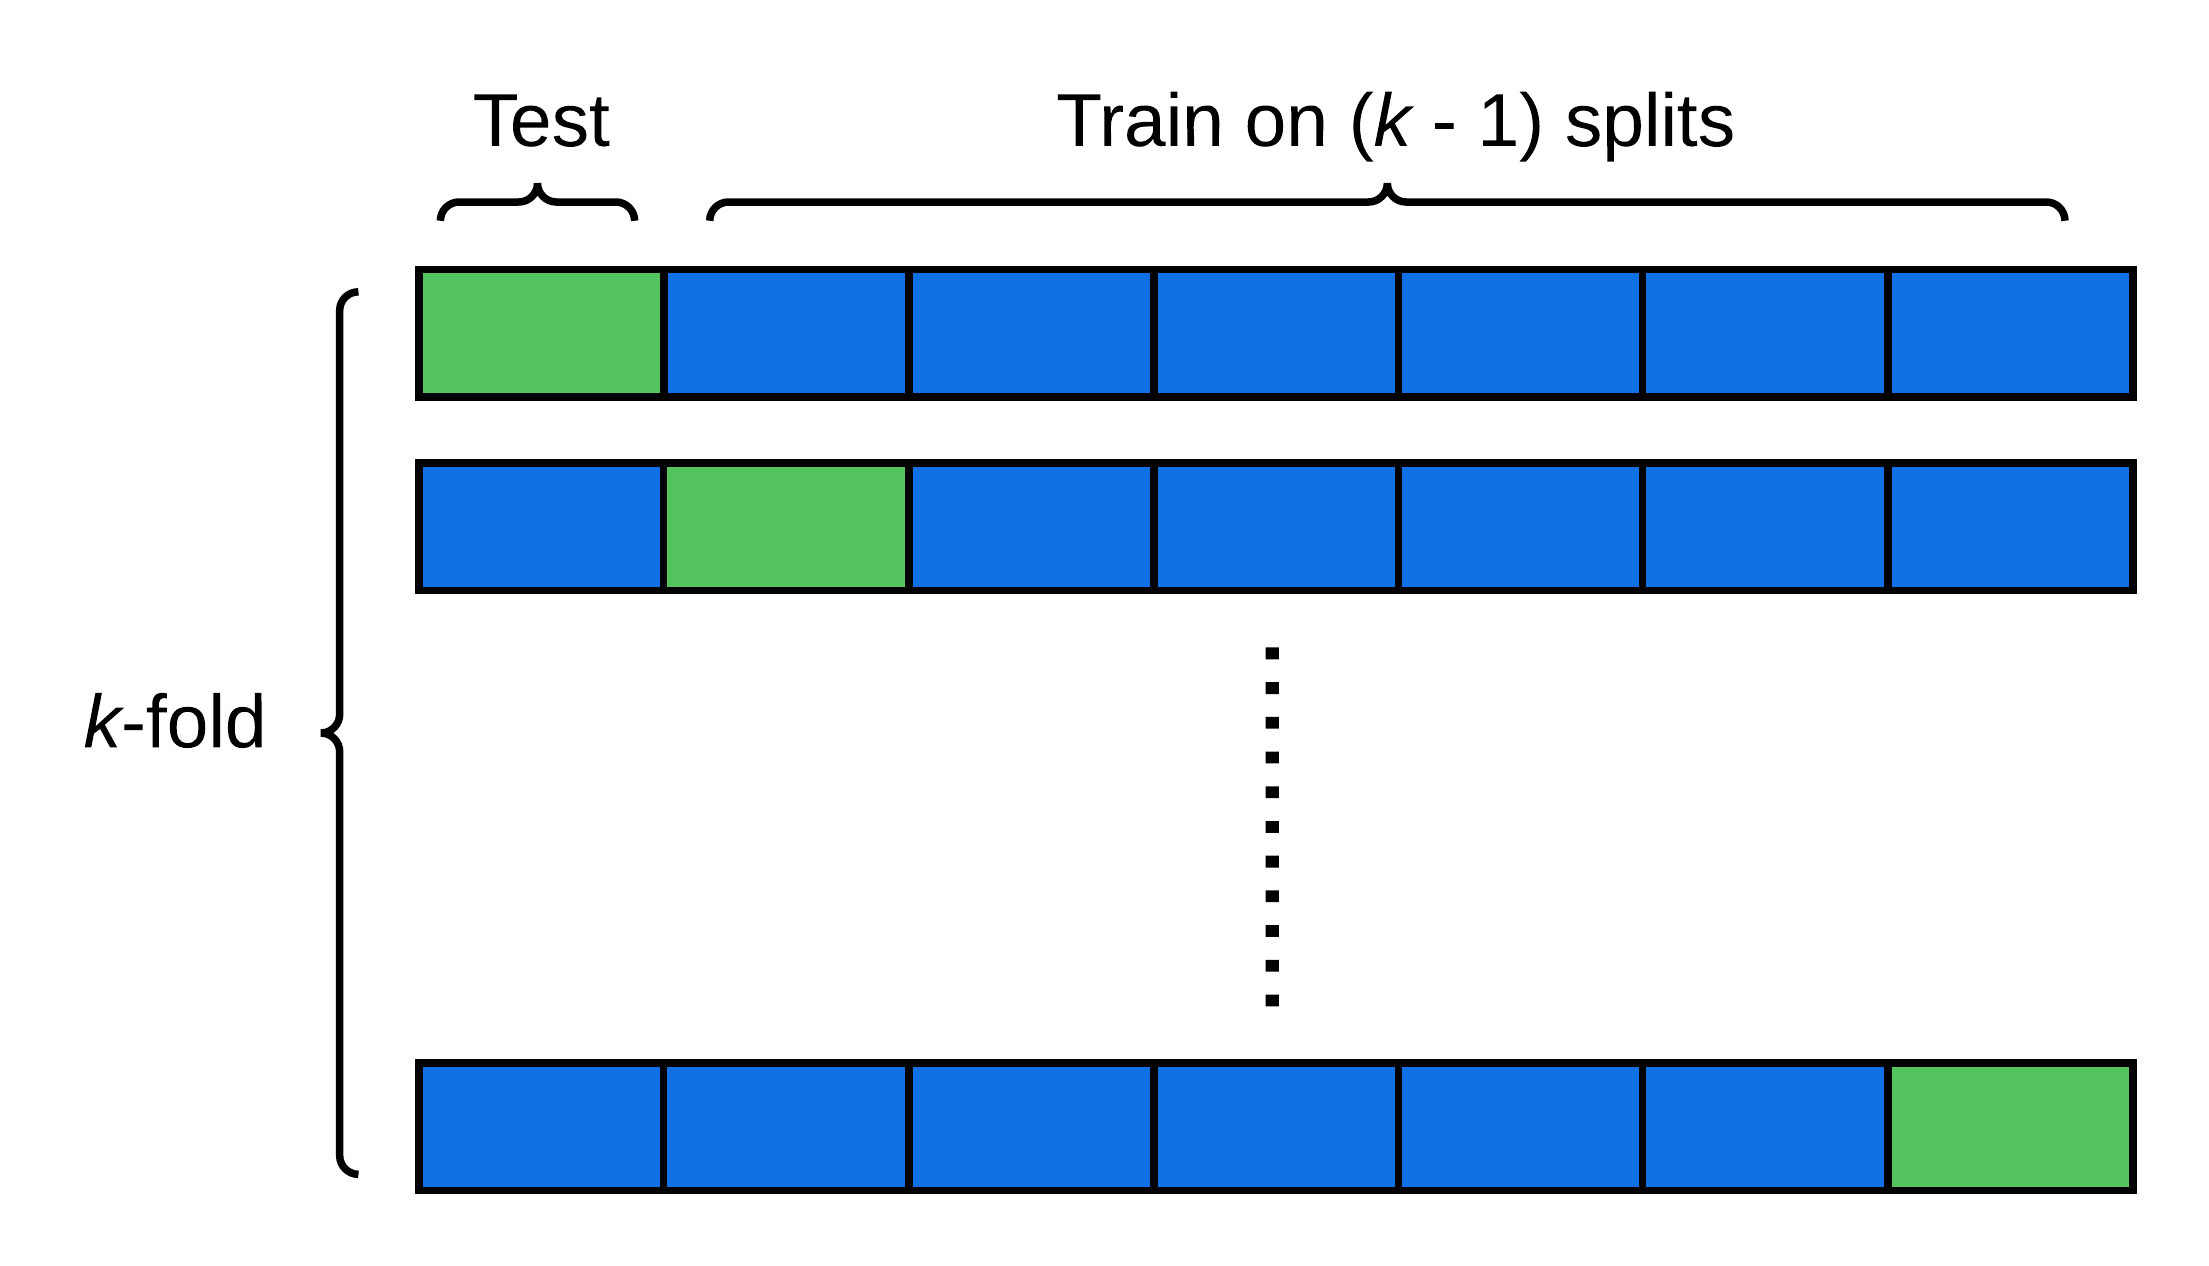
\includegraphics[width=\linewidth]{graphics/LOOCV.png}
    \caption{LOOCV algorithm example on \textit{k} folds}
    \label{fig:LOOCV}
\end{figure}

\subsubsection{Evaluation Metrics}
Confusion matrix
Roc curve e AUC




